% 第 12 周交付物：结项报告（中文版）——在第 8 周最终报告（docs/week8/final_report_cn.tex，原文件保留）上续写第 9--12 周
% 编译方式：XeLaTeX，三遍。第 9--12 周的全部数字来自 numbers.tex（由 analysis/week12/04_report_numbers.py 从各周输出生成）
\documentclass[11pt]{ctexart}
\usepackage[a4paper, margin=2.4cm]{geometry}
\usepackage{amsmath, amssymb}
\usepackage{booktabs}
\usepackage{graphicx}
\usepackage[hidelinks]{hyperref}
\usepackage{enumitem}
\setlist{nosep}
\usepackage{parskip}
\usepackage{float}
% generated by analysis/week12/04_report_numbers.py - do not edit by hand
\newcommand{\rnWnineQuoteMs}{1.8}
\newcommand{\rnWnineRedisMs}{0.15}
\newcommand{\rnWnineRenderMs}{724}
\newcommand{\rnWnineDailyS}{4.5}
\newcommand{\rnMemIntervals}{670}
\newcommand{\rnMemTickers}{666}
\newcommand{\rnPanelTenRows}{617{,}211}
\newcommand{\rnPanelTenTickers}{532}
\newcommand{\rnEone}{9.5}
\newcommand{\rnEtwo}{6.8}
\newcommand{\rnEthree}{5.4}
\newcommand{\rnEfour}{163.8}
\newcommand{\rnEfive}{69.9}
\newcommand{\rnTenDailyS}{38.0}
\newcommand{\rnGoneDWin}{72}
\newcommand{\rnGoneDPooled}{0.812}
\newcommand{\rnRoundOneRidge}{7.16}
\newcommand{\rnRoundOneGbdt}{2.23}
\newcommand{\rnNoPrices}{51}
\newcommand{\rnInStudy}{597}
\newcommand{\rnTruncated}{3}
\newcommand{\rnPostExit}{7}
\newcommand{\rnLatestBeforeMs}{457}
\newcommand{\rnLatestBeforeRows}{579}
\newcommand{\rnLatestFinalMs}{0.3}
\newcommand{\rnLatestFinalRows}{1496}
\newcommand{\rnQuBeforeMs}{390}
\newcommand{\rnQuBeforeN}{578}
\newcommand{\rnQuAfterMs}{23.5}
\newcommand{\rnQuAfterN}{1496}
\newcommand{\rnMarketBeforeS}{12.8}
\newcommand{\rnMarketAfterS}{2.6}
\newcommand{\rnFeatBeforeS}{14.7}
\newcommand{\rnFeatAfterS}{14.5}
\newcommand{\rnDailyAfterS}{25.8}
\newcommand{\rnScaleSteadyS}{59.5}
\newcommand{\rnScaleN}{1517}
\newcommand{\rnScaleBackfillS}{530}
\newcommand{\rnRenderBeforeMs}{591}
\newcommand{\rnRenderAfterMs}{514}
\newcommand{\rnFinalQuMs}{50}
\newcommand{\rnFinalQuN}{1496}
\newcommand{\rnFinalScalarMs}{27}
\newcommand{\rnFinalXsMs}{27}
\newcommand{\rnFinalRenderMs}{510}
\newcommand{\rnGarchOrdS}{3.2}
\newcommand{\rnGarchRefitS}{15.2}
\newcommand{\rnGarchRefits}{1{,}326}
\newcommand{\rnGarchTickers}{1{,}479}
\newcommand{\rnCatchupS}{84.4}
\newcommand{\rnCatchupFeatS}{62.7}
\newcommand{\rnDbFinalMb}{1601}
\newcommand{\rnDbElevenMb}{1570}
\newcommand{\rnRssFinalMb}{299}
\newcommand{\rnRssElevenMb}{286}
\newcommand{\rnElevenTestMl}{0.755}
\newcommand{\rnElevenTestG}{0.791}
\newcommand{\rnElevenMaeMl}{7.91}
\newcommand{\rnElevenMaeG}{8.36}
\newcommand{\rnElevenMaeE}{10.35}
\newcommand{\rnElevenVal}{0.705}
\newcommand{\rnElevenTestStart}{2024-05-24}
\newcommand{\rnNoDummyTest}{0.741}
\newcommand{\rnUnknownN}{52}
\newcommand{\rnUnknownRemoved}{51}
\newcommand{\rnGTrain}{0.840}
\newcommand{\rnGVal}{0.777}
\newcommand{\rnCsOnly}{0.742}
\newcommand{\rnLevelOnly}{0.801}
\newcommand{\rnOosStart}{2022-12-27}
\newcommand{\rnOosEnd}{2024-12-31}
\newcommand{\rnOosDates}{506}
\newcommand{\rnOosRows}{244{,}038}
\newcommand{\rnOosTickers}{505}
\newcommand{\rnOosMaeE}{7.55}
\newcommand{\rnOosMaeG}{6.49}
\newcommand{\rnOosMaeMl}{6.15}
\newcommand{\rnHOneDelta}{1.07}
\newcommand{\rnHOneLo}{0.65}
\newcommand{\rnHOneHi}{1.62}
\newcommand{\rnHOneSizeTicker}{48}
\newcommand{\rnHOneSizeSector}{9.3}
\newcommand{\rnHOnePholm}{0.002}
\newcommand{\rnHTwoDelta}{0.337}
\newcommand{\rnHTwoLo}{0.206}
\newcommand{\rnHTwoHi}{0.456}
\newcommand{\rnHTwoSizeTicker}{50}
\newcommand{\rnHTwoSizeSector}{4.7}
\newcommand{\rnHTwoPholm}{0.002}
\newcommand{\rnHThreeDelta}{1.48}
\newcommand{\rnHThreeLo}{1.15}
\newcommand{\rnHThreeHi}{1.80}
\newcommand{\rnHThreeSizeTicker}{23}
\newcommand{\rnHThreeSizeSector}{3.7}
\newcommand{\rnHThreePholm}{0.002}
\newcommand{\rnHFourDelta}{1.77}
\newcommand{\rnHFourLo}{1.29}
\newcommand{\rnHFourHi}{2.44}
\newcommand{\rnHFourSizeTicker}{42}
\newcommand{\rnHFourSizeSector}{8.0}
\newcommand{\rnHFourPholm}{0.002}
\newcommand{\rnHTwoYThree}{0.048}
\newcommand{\rnHTwoYFour}{0.634}
\newcommand{\rnHTwoBDelta}{0.286}
\newcommand{\rnSelfIidTicker}{6.7}
\newcommand{\rnSelfShockTicker}{69}
\newcommand{\rnSelfShockSector}{9.3}
\newcommand{\rnIvJpm}{0.710}
\newcommand{\rnIvJpmCorr}{0.78}
\newcommand{\rnIvJpmCorrConst}{0.83}
\newcommand{\rnIvPanelRows}{467{,}189}
\newcommand{\rnIvPanelTickers}{506}
\newcommand{\rnIvMaeIv}{5.16}
\newcommand{\rnIvMaeGd}{6.63}
\newcommand{\rnIvMaeGy}{6.92}
\newcommand{\rnIvMaeRv}{7.60}
\newcommand{\rnIvMaeEw}{7.52}
\newcommand{\rnIvWinGd}{92}
\newcommand{\rnIvWinGy}{70}
\newcommand{\rnIvConstIv}{4.69}
\newcommand{\rnIvConstGy}{6.47}
\newcommand{\rnIvXsIv}{0.95}
\newcommand{\rnIvXsGy}{0.84}
\newcommand{\rnIvTsIv}{0.11}
\newcommand{\rnIvGapActual}{1.77}
\newcommand{\rnIvGapConst}{1.78}
\newcommand{\rnBandGCalm}{5.48}
\newcommand{\rnBandGFear}{5.86}
\newcommand{\rnBandESameCalm}{6.66}
\newcommand{\rnBandESameFear}{4.89}
\newcommand{\rnBandEFullCalm}{9.01}
\newcommand{\rnBandEFullFear}{10.83}
\newcommand{\rnBandGDays}{1011}
\newcommand{\rnToolAsOf}{2026-10-02}
\newcommand{\rnToolQuoted}{1{,}493}
\newcommand{\rnToolGarch}{1{,}478}
\newcommand{\rnToolEwma}{15}
\newcommand{\rnToolMl}{496}


\title{\textbf{Advanced Chooser Option Pricing Model\\ with Real-World Data \& Machine Learning}\\
\Large 结项报告}
\author{佟铸城（Zhucheng Tong）}
\date{2026 年 10 月 13 日 \quad（项目周期：2026-07 至 2026-10，第 1--12 周）}

\begin{document}
\maketitle

\begin{abstract}
本项目围绕 JPM 标的的 simple chooser option 构建了一套数据驱动的定价体系：复现并三角验证了 Rubinstein（1991）闭式解与蒙特卡洛定价，在 1310 个交易日的真实数据上以“事后真值”口径量化了 BSM 常数波动率假设的代价（最优回望校准的相对误差约 35\%），继而在严格的样本外协议（净化时序切分、walk-forward 重训、测试集单次开封）下检验了两条机器学习增强路线。核心结论：（1）失效模式随波动率估计器记忆长度分化，无单一回望窗口全状态占优；（2）在仅含约一个半波动率状态周期的训练数据上，ML 修正无法稳健标定，所有配置在测试集上不敌 EWMA 锚定基线——该负结果经六项审计确认为科学结论而非实现缺陷；（3）正确的融合形态是“随机过程出框架、机器学习学残差”的 1+1 结构而非二选一。第 8 周的交付物为一个 Streamlit 双定价工具：主定价采用当时最稳健的 EWMA 锚定 BSM，ML 修正价附样本外警示作参考。

第 9--12 周（enhancement 阶段）按导师给出的三个方向推进：把数据管道与工具搬上 PostgreSQL + Redis + Docker 的在线栈并由调度器每日自动更新；把标的从 JPM 扩展到点时重建的 S\&P 500 成分股（压测扩至 S\&P 1500）并完成全流程性能剖析与优化；理论线在面板上重新检验锚与机器学习。结项结论：（1）GARCH(1,1) 1 日预测作为锚，在训练、验证、测试三个窗口都优于 EWMA，已替换为工具的主定价锚；（2）横截面锚定 ML 在 2023--2024 年样本外相对 GARCH 锚的增量为每份 \rnHTwoDelta{} 美元 MAE（95\% 区间 \rnHTwoLo{}--\rnHTwoHi），判据、size 检验与多重比较矫正均事先登记——该区间以这段时期为条件，时间维度上只有两个独立年份，不足以做时间上的显著性推断；据此按事先规则把 ML 参考价扩展到面板成员；（3）隐含波动率在面板上是检验过的最强的锚（MAE \rnIvMaeIv{} 美元，GARCH 1 日锚 \rnIvMaeGd），优势来自对每只股票波动率水平的定位而非择时，但按预注册判据只能定位为研究基准：它对免费平稳锚的优势未能通过合格的推断程序，公开数据源的可部署性也无法核实。
\end{abstract}

\clearpage
{\small\setlength{\parskip}{0pt}\tableofcontents}
\newpage

\section{项目概述}
Chooser option 赋予持有人在选择日 $t_1$ 决定期权为欧式 call 或 put 的权利（共同行权价 $K$、到期日 $T_2$），适用于方向不明但预期大波动的场景（财报、FOMC 等）。项目目标：（1）复现参考论文（Huang, Wang \& Wan, 2021）的 BSM 定价并以真实数据验证；（2）多维数据采集与特征工程；（3）机器学习优化波动率预测与定价；（4）量化 ML 与传统 BSM 的对比；（5）交付可部署定价工具。八周执行路线：数据管道（W1--2）$\to$ 复现与基线（W3--4）$\to$ ML 两路线（W5--6）$\to$ 工具与交付（W7--8）。

\section{数据体系（第 1--2 周）}
\textbf{来源}：Yahoo Finance（JPM 日线含股息、\^{}GSPC、\^{}VIX、国债收益率指数，主源）、FRED（DGS3MO/DGS1/DGS10/FEDFUNDS/T10Y2Y）、Alpha Vantage（备用/实时）；窗口 2018--2024 日频，经导师确认以 VIX 派生特征替代新闻情绪数据、以蒙特卡洛替代 CME 成交价。\textbf{清洗}：NYSE 交易日历对齐、按缺失机制区分的填充（利率时间插值、政策利率阶梯填充）、IQR 离群值\textbf{标记但保留}（全部对应真实市场事件，审计留档）。\textbf{特征}：18 个，分收益/波动率、股息、利率、市场背景、情绪（VIX 派生，0--1 情绪分 = 滚动 252 日分位；双重角色控制：原始水平=波动率、标准化变换=情绪）五族。\textbf{自动化}：GitHub Actions 每周五收盘后自动采集$\to$预处理$\to$提交，研究窗口与数据新鲜度经环境变量解耦。

\section{Chooser 定价理论与复现（第 3 周）}
利用 put--call parity，simple chooser 在 $t_1$ 的价值 $\max(C,P)$ 可分解为静态组合：一份 $(K,T_2)$ call 加 $e^{-q\tau}$ 份 $(Ke^{-(r-q)\tau},t_1)$ put（$\tau=T_2-t_1$），故 BSM 下存在闭式解。以论文 Table 2 参数（$S_0=156.7$，$K=150$，$r=0.15\%$，$\sigma=28.2\%$，$q=2.33\%$，$t_1=0.5$，$T_2=1$）复现：

\begin{center}
\small
\begin{tabular}{lr}
\toprule
闭式解（两种独立实现，差异 $7\times10^{-15}$） & \textbf{\$29.1299} \\
蒙特卡洛（条件 MC，100 万路径） & \$29.1426 $\pm$ 0.0165 \\
vanilla call / put / straddle & \$18.69 / \$15.37 / \$34.06 \\
\bottomrule
\end{tabular}
\end{center}

正确性由三角测量确立：双解析实现互查、双 MC 估计量（$1/\sqrt{n}$ 收敛）、无套利排序 $\max(C,P)<\text{chooser}<\text{straddle}$。条件 MC（选择日价值解析化）使标准误降至终值模拟的 54\%。论文的四条敏感性方向全部复现；两项超出论文的增量：（a）$t_1$ 敏感性（论文自认未竟）——价值从 $\max(C,P)$ 单调过渡到 straddle；（b）论文 moneyness 选择规则（理性临界点应为 $S^*=Ke^{(q-r)\tau}$ 而非 $K$）的代价量化：2021 年零利率下仅 6bp、$r=10\%$ 时放大至 60bp，真实日期复检 14.4bp $\to$ 32.2bp——近似是否无害是状态依赖的命题。

\begin{figure}[H]
\centering
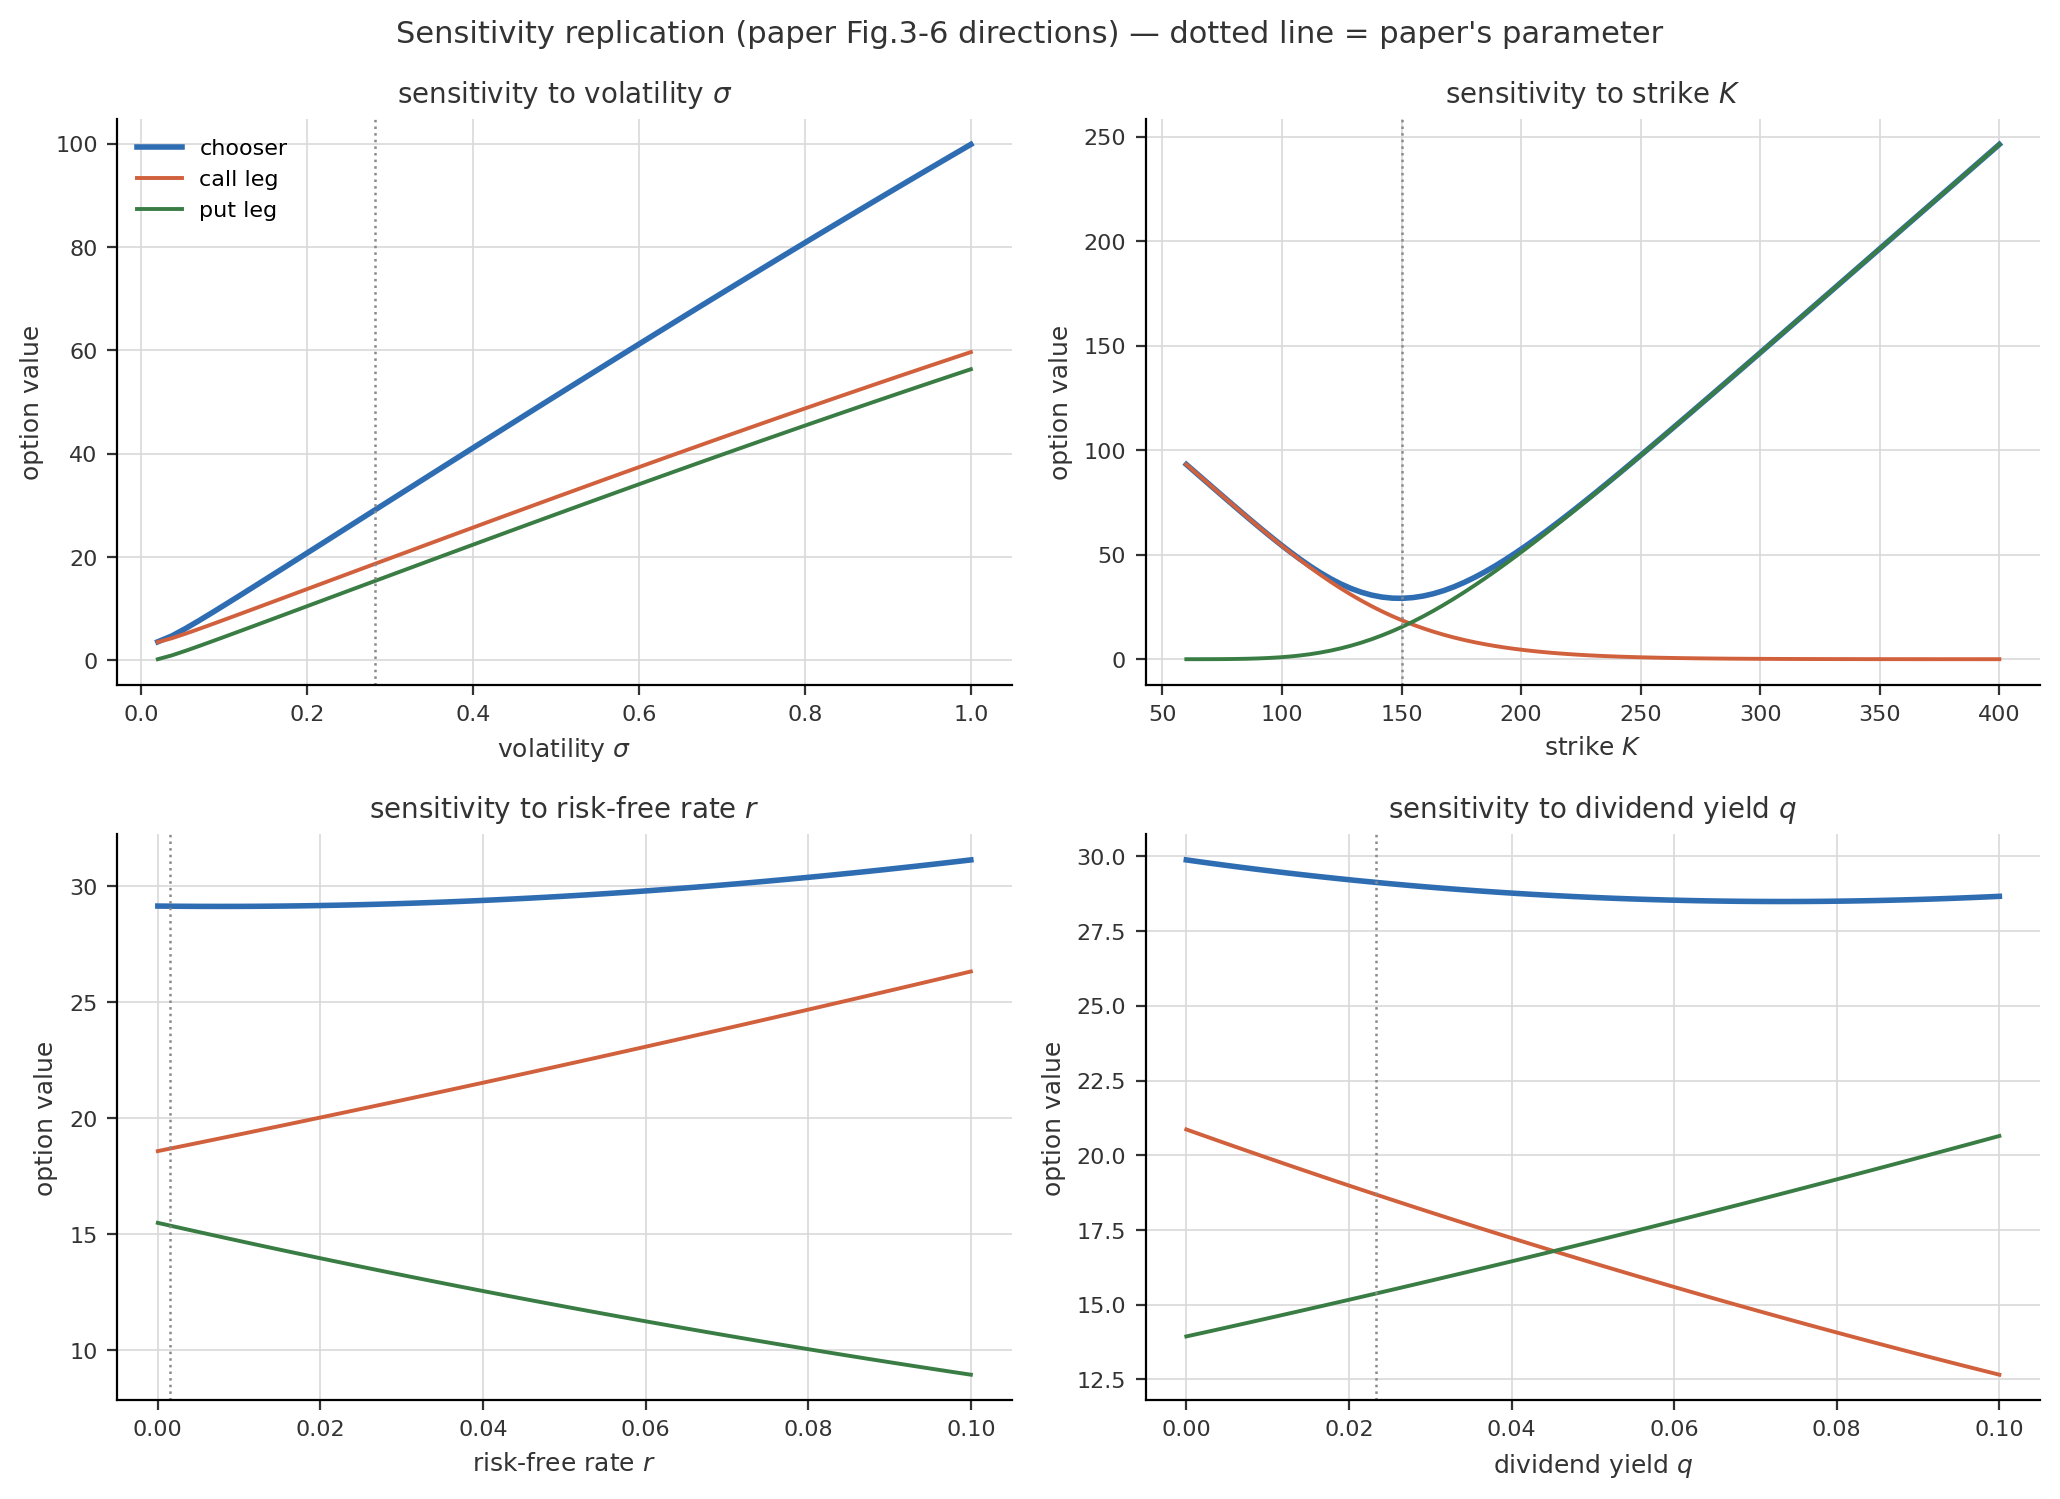
\includegraphics[width=0.9\textwidth]{../week3/figures/sensitivity_panels.png}
\caption{敏感性复现（$\sigma$/$K$/$r$/$q$；虚线为论文参数点）：方向与论文 Fig.3--6 一致，chooser 对 $K$ 呈 U 形}
\end{figure}

\begin{figure}[H]
\centering
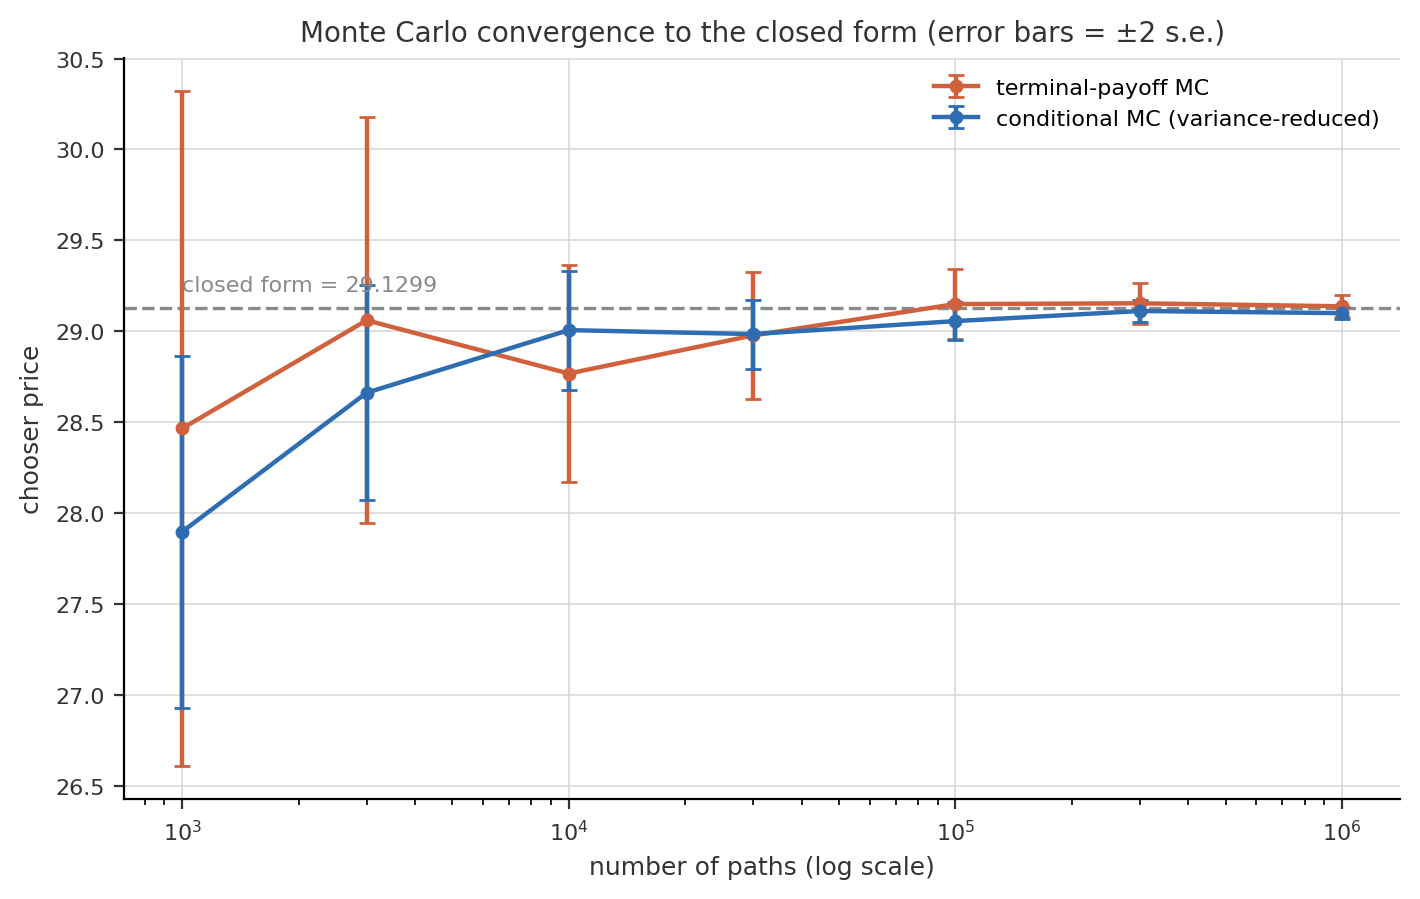
\includegraphics[width=0.58\textwidth]{../week3/figures/convergence.png}
\caption{MC 收敛性：条件 MC 与终值模拟均以 $1/\sqrt{n}$ 收敛于闭式解}
\end{figure}

\section{基线评估：常数波动率假设的代价（第 4 周）}
评估设计采用\textbf{事后真值（oracle）}口径：逐日发行 ATM 1 年期 chooser，回望校准价（$\sigma$ 取各回望估计器）与“用存续期内实际实现波动率”的 oracle 价对比——误差唯一地归因于常数波动率假设。样本 1310 个交易日（2019-10 至 2024-12）。

\begin{center}
\small
\begin{tabular}{lrrrrr}
\toprule
\textbf{$\sigma$ 估计器} & \textbf{MAE(\$)} & \textbf{相对 MAE} & \textbf{平静期} & \textbf{恐慌期} & \textbf{综合分} \\
\midrule
21 日已实现 & 9.80 & 36.1\% & 9.31 & 11.38 & 1.067 \\
63 日已实现 & 9.76 & 37.4\% & 9.47 & 10.70 & 0.994 \\
252 日已实现 & 10.37 & 41.7\% & \textbf{10.94} & 8.55 & 0.982 \\
EWMA($\lambda$=0.94) & \textbf{9.44} & \textbf{35.3\%} & 9.01 & 10.83 & 1.000（参照）\\
\bottomrule
\end{tabular}
\end{center}

关键发现：（1）最优回望校准的代价仍达价格的 \textbf{35\%}；（2）\textbf{失效模式随记忆长度分化}——快估计器（21日/EWMA）在恐慌期追高失效，252 日慢估计器在危机后的平静期拖尾失效（2021 年：\$10.34 vs 21 日的 \$6.13），无单一窗口全状态占优；（3）所有回望基线对 oracle 价格的 $R^2$ 为负（约 $-1.1$），解释力不如常数均值——常数波动率失效的最尖锐表述；（4） 2019 年尾段误差（\$31.8）源于标签窗口内的 COVID 崩盘，为任何回望方法（含 ML）设定了不可约的期望上限。
\begin{figure}[H]
\centering
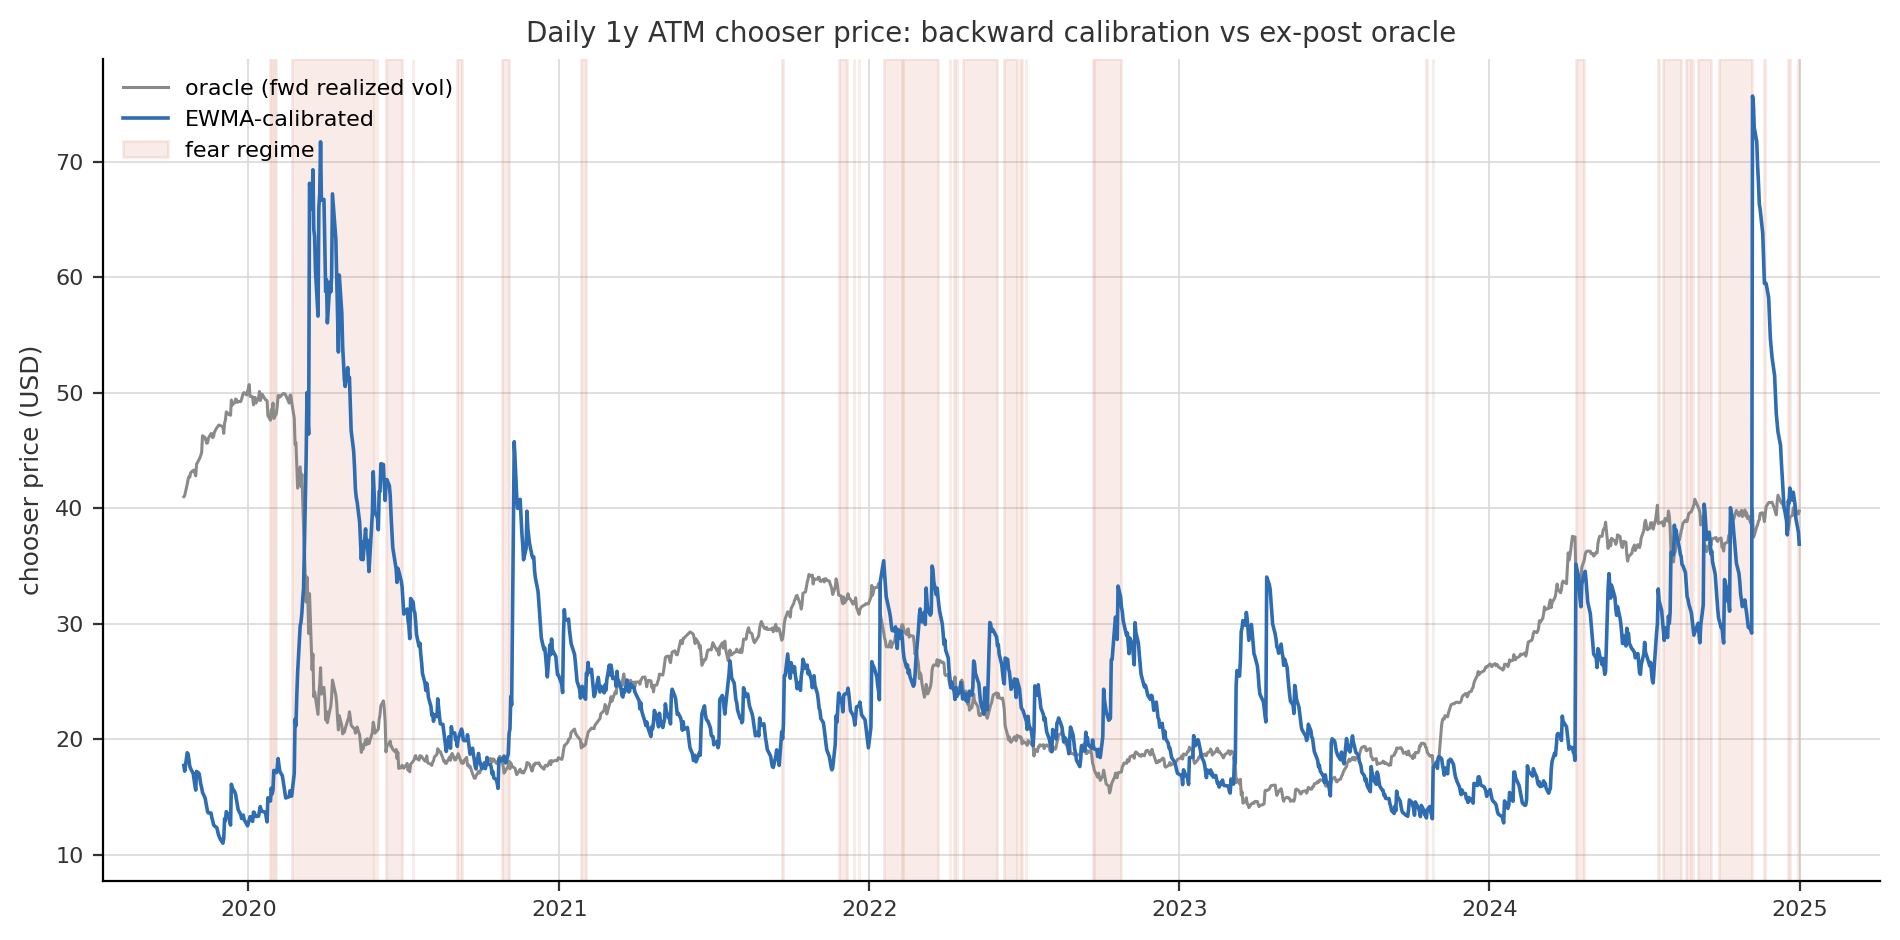
\includegraphics[width=0.94\textwidth]{../week4/figures/rolling_price.png}
\caption{逐日定价：EWMA 回望校准（蓝） vs 事后真值（灰），阴影为恐慌状态——2020 年初灰线先行抬升而蓝线浑然不觉，即 BSM 危机前低估、危机后高估}
\end{figure}

\begin{figure}[H]
\centering
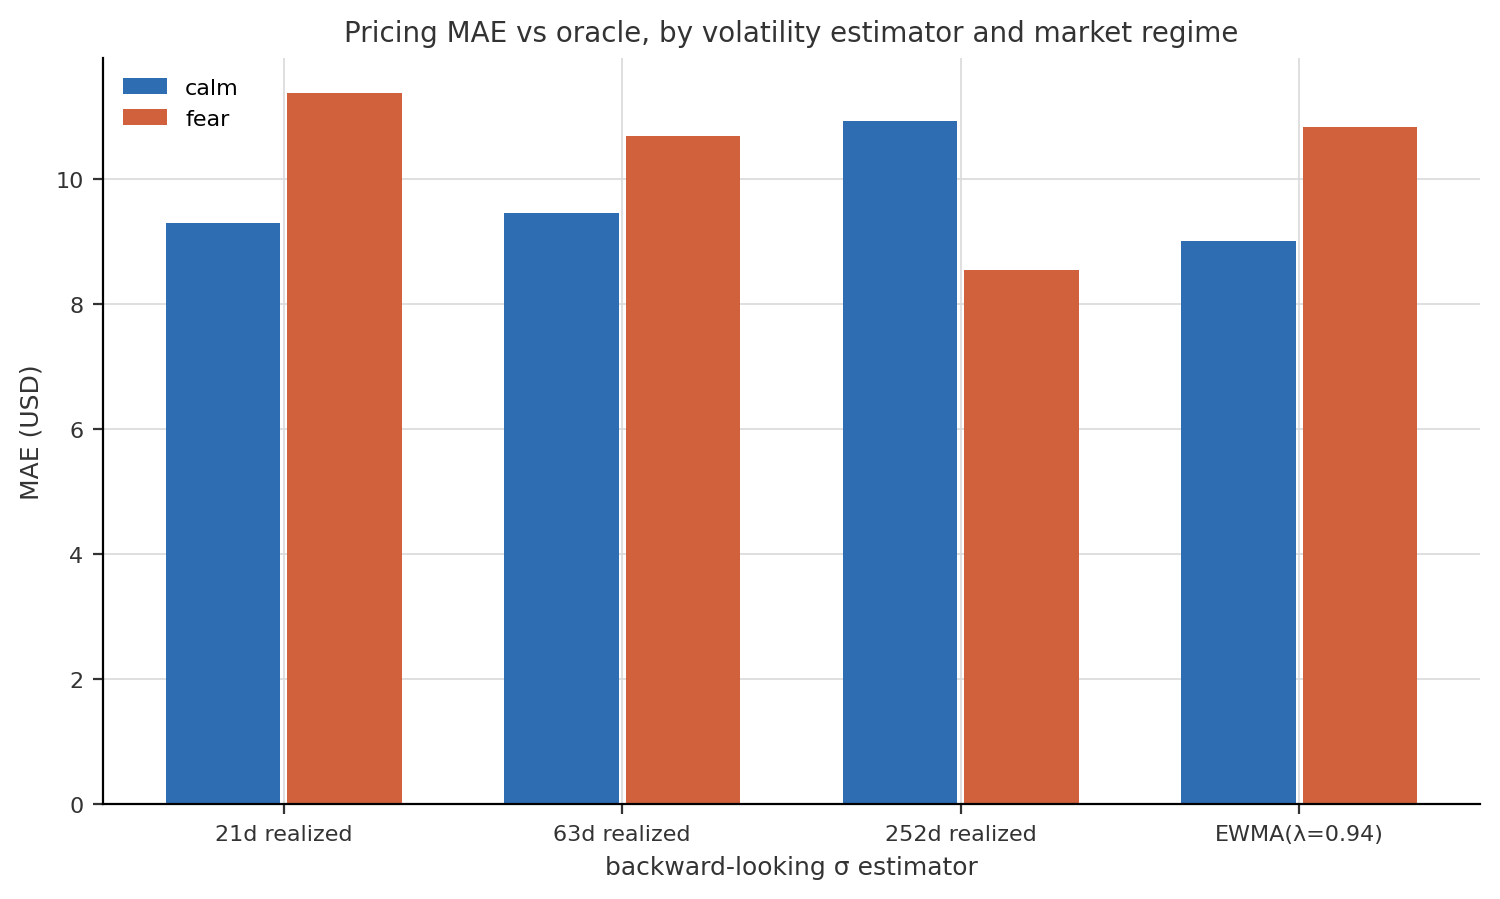
\includegraphics[width=0.6\textwidth]{../week4/figures/mae_by_regime.png}
\caption{分状态 MAE：快估计器恐慌期更差、252 日估计器平静期更差}
\end{figure}

\subsection{评估指标体系（应导师要求扩展，全项目同一把尺）}
\begin{center}
\small
\begin{tabular}{llp{6.6cm}r}
\toprule
\textbf{指标族} & \textbf{指标} & \textbf{衡量什么} & \textbf{权重} \\
\midrule
平均精度 & MAE / RMSE / MedAE & 常规误差；中位数对极端日不敏感 & 0.35 \\
尾部/稳健 & P95AE / 分状态最差 MAE & 最差 5\% 交易日；不许牺牲某一状态换平均 & 0.30 \\
方向偏差 & $|$Bias$|$ & 系统性高估/低估，对报价比对称噪声更危险 & 0.10 \\
解释力 & $1-R^2$ & 相对“永远猜均值”的改进 & 0.10 \\
可用率 & $1-$Hit10 & 相对误差 $<10\%$ 的天数占比 & 0.15 \\
\bottomrule
\end{tabular}
\end{center}
综合分 $=\sum_i w_i\,\mathrm{metric}_i(m)/\mathrm{metric}_i(\text{EWMA})$，参照模型恒为 1、$<1$ 即胜基线；比值化使新增模型无需重新归一，并附等权/精度导向/稳健导向三种替代权重的排名敏感性检验。

\section{机器学习增强：设计、协议与结果（第 5--6 周）}

\subsection{防泄漏协议}
70/15/15 时序切分 + \textbf{净化}（训练尾部删 252 行，标签前视窗不越界）+ 测试集（2024-03 至 2024-12）\textbf{单次开封}（全部选择只用验证集，审计断言保证选择日志零测试信息）+ walk-forward 季度重训（逐块净化与 scaler 重拟合）。

\subsection{设计演进：从水平目标到锚定目标}
直接预测波动率水平的七个初版模型（Ridge/RF/GBDT/LSTM $\times$ 两路线）在验证集\textbf{全军覆没}（综合分 2.0--3.7，统一正偏差 $+14$ 至 $+26$ 美元）：COVID 主导的训练窗遇上低波动验证窗，树模型无法输出低于训练所见的值。修正为\textbf{锚定目标} $y=\ln(\sigma_{oracle}/\sigma_{EWMA})$（输出 0 恒等还原基线，审计断言逐日验证）后，锚定 Ridge 在验证集综合分 0.567、首个全面击败基线——锚定与第 3 周条件 MC 同源：\textbf{把已知结构从任务中剥离，学习只留给残差}。

\begin{figure}[!htb]
\centering
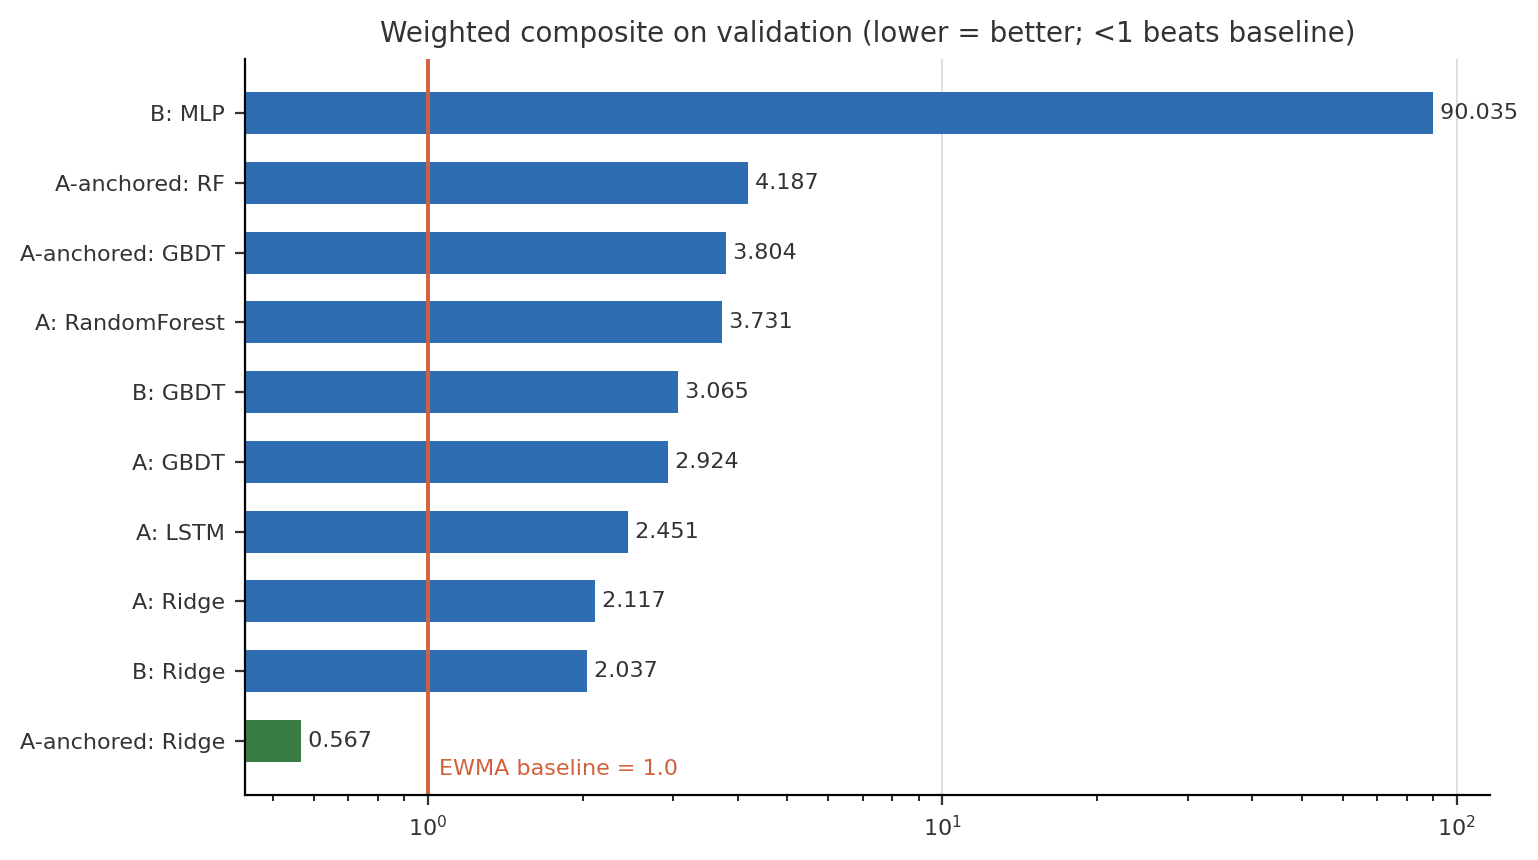
\includegraphics[width=0.72\textwidth]{../week5/figures/val_composite.png}
\caption{第 5 周验证集综合分（对数轴）：锚定 Ridge（绿，0.567）为唯一 $<1$ 者；直接预测水平的模型全部大幅劣于基线}
\end{figure}

\subsection{调参（仅用验证集）}
\begin{center}
\small
\begin{tabular}{llr}
\toprule
\textbf{模型} & \textbf{选中超参数} & \textbf{验证 MAE(\$)} \\
\midrule
A: Ridge / B: Ridge & $\alpha=10$ / $\alpha=10$ & 10.77 / 11.09 \\
A: RandomForest & max\_depth=4 & 20.35 \\
A: GBDT / B: GBDT & lr=0.03，200 轮 / lr=0.05，300 轮 & 24.17 / 23.33 \\
A: LSTM（固定配置） & hidden 32 & \textbf{2.82} \\
B: MLP（鲁棒化） & （64,32），输入裁剪 & 12.12 \\
\bottomrule
\end{tabular}
\end{center}

\subsection{最终样本外结果：一个如实报告的负结果}
经调参与 walk-forward 后在测试集单次评估：

\begin{center}
\small
\begin{tabular}{lrrrr}
\toprule
& \textbf{MAE(\$)} & \textbf{Bias} & \textbf{Hit10} & \textbf{综合分} \\
\midrule
\textbf{EWMA 基线} & \textbf{8.51} & $-3.4$ & \textbf{26.8\%} & \textbf{1.000} \\
最优 ML（鲁棒 MLP） & 14.75 & $+14.3$ & 13.6\% & 2.020 \\
验证集冠军（LSTM，val MAE 2.82） & 17.07 & $+16.6$ & 13.6\% & 2.492 \\
其余五个配置 & 20.5--22.0 & $+20$ 上下 & $\leq10.6\%$ & 2.56--2.83 \\
\bottomrule
\end{tabular}
\end{center}

\textbf{没有任何 ML 配置在测试集上击败 EWMA 基线}（四种权重方案下均然）。归因三条：（1）锚定比率目标具强低频状态自相关，训练数据仅含约一个半状态轮换，模型学到的是“上一个状态”；（2）测试期全部标签窗口覆盖 2025-04 崩盘（不可预见，EWMA 胜在不试图预测）；（3）事后诊断（如实标注、未用于选择）表明第 5 周验证集胜利部分源于训练分布与验证需求的巧合——\textbf{单一验证窗的胜利不构成部署证据}。验证集冠军 LSTM 的测试劣化（2.82 $\to$ 17.07）是教科书式验证集过拟合实例。SHAP 显示模型学到干净的均值回复逻辑（方向正确），失败在幅度不可标定——瓶颈是数据中可辨认的状态样本数，而非算法。该负结果与“单纯时序暴力拟合不如定价模型推导精确”的判断一致，并直接决定了工具的定价策略。

\begin{figure}[H]
\centering
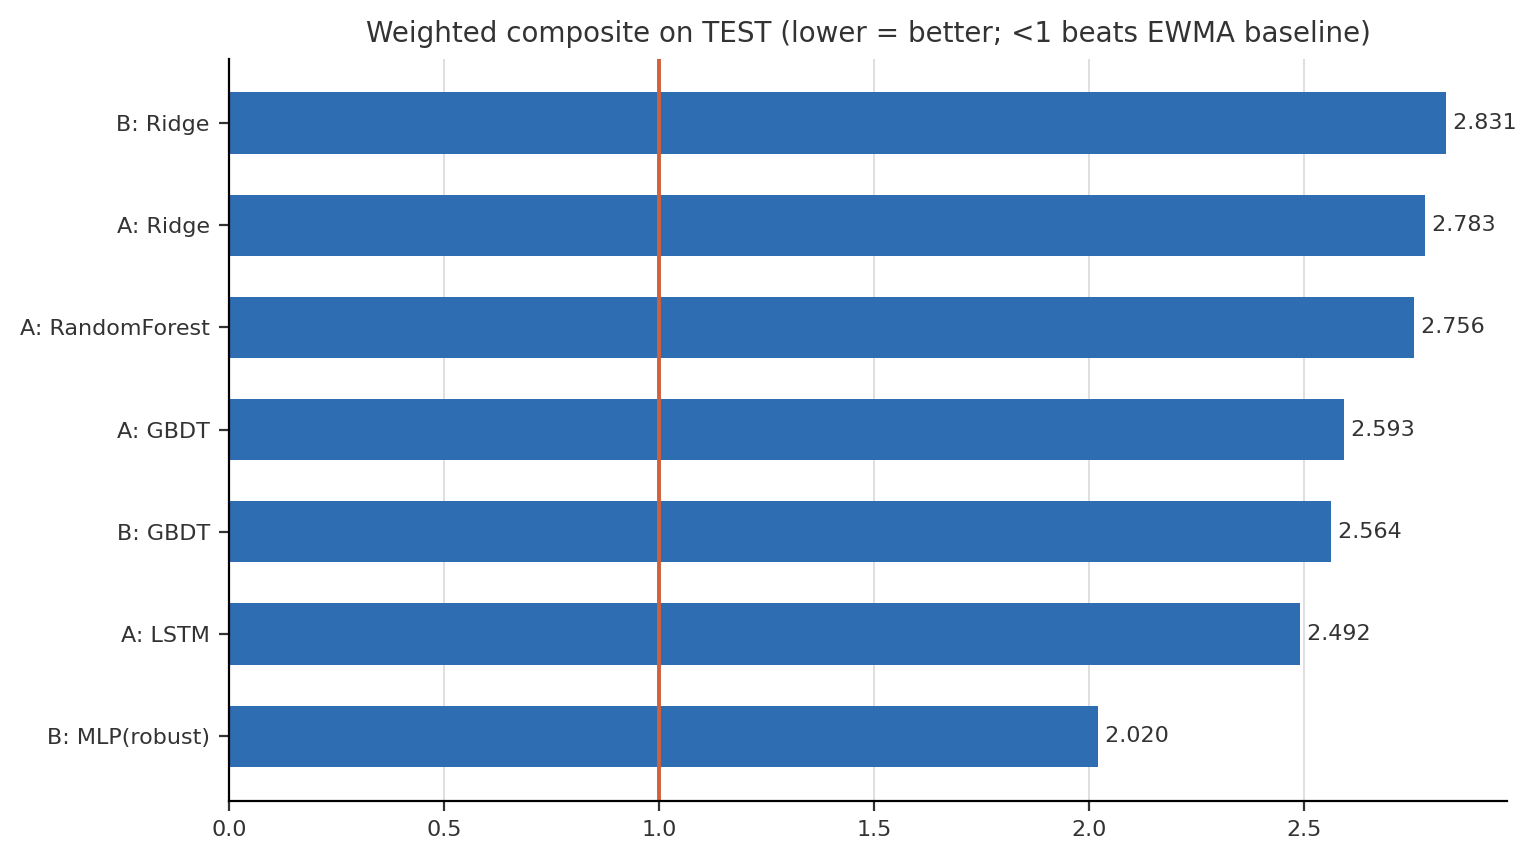
\includegraphics[width=0.7\textwidth]{../week6/figures/test_composite.png}
\caption{测试集综合分：全部 ML $>1$，EWMA 基线四种权重方案下均胜出}
\end{figure}

\begin{figure}[H]
\centering
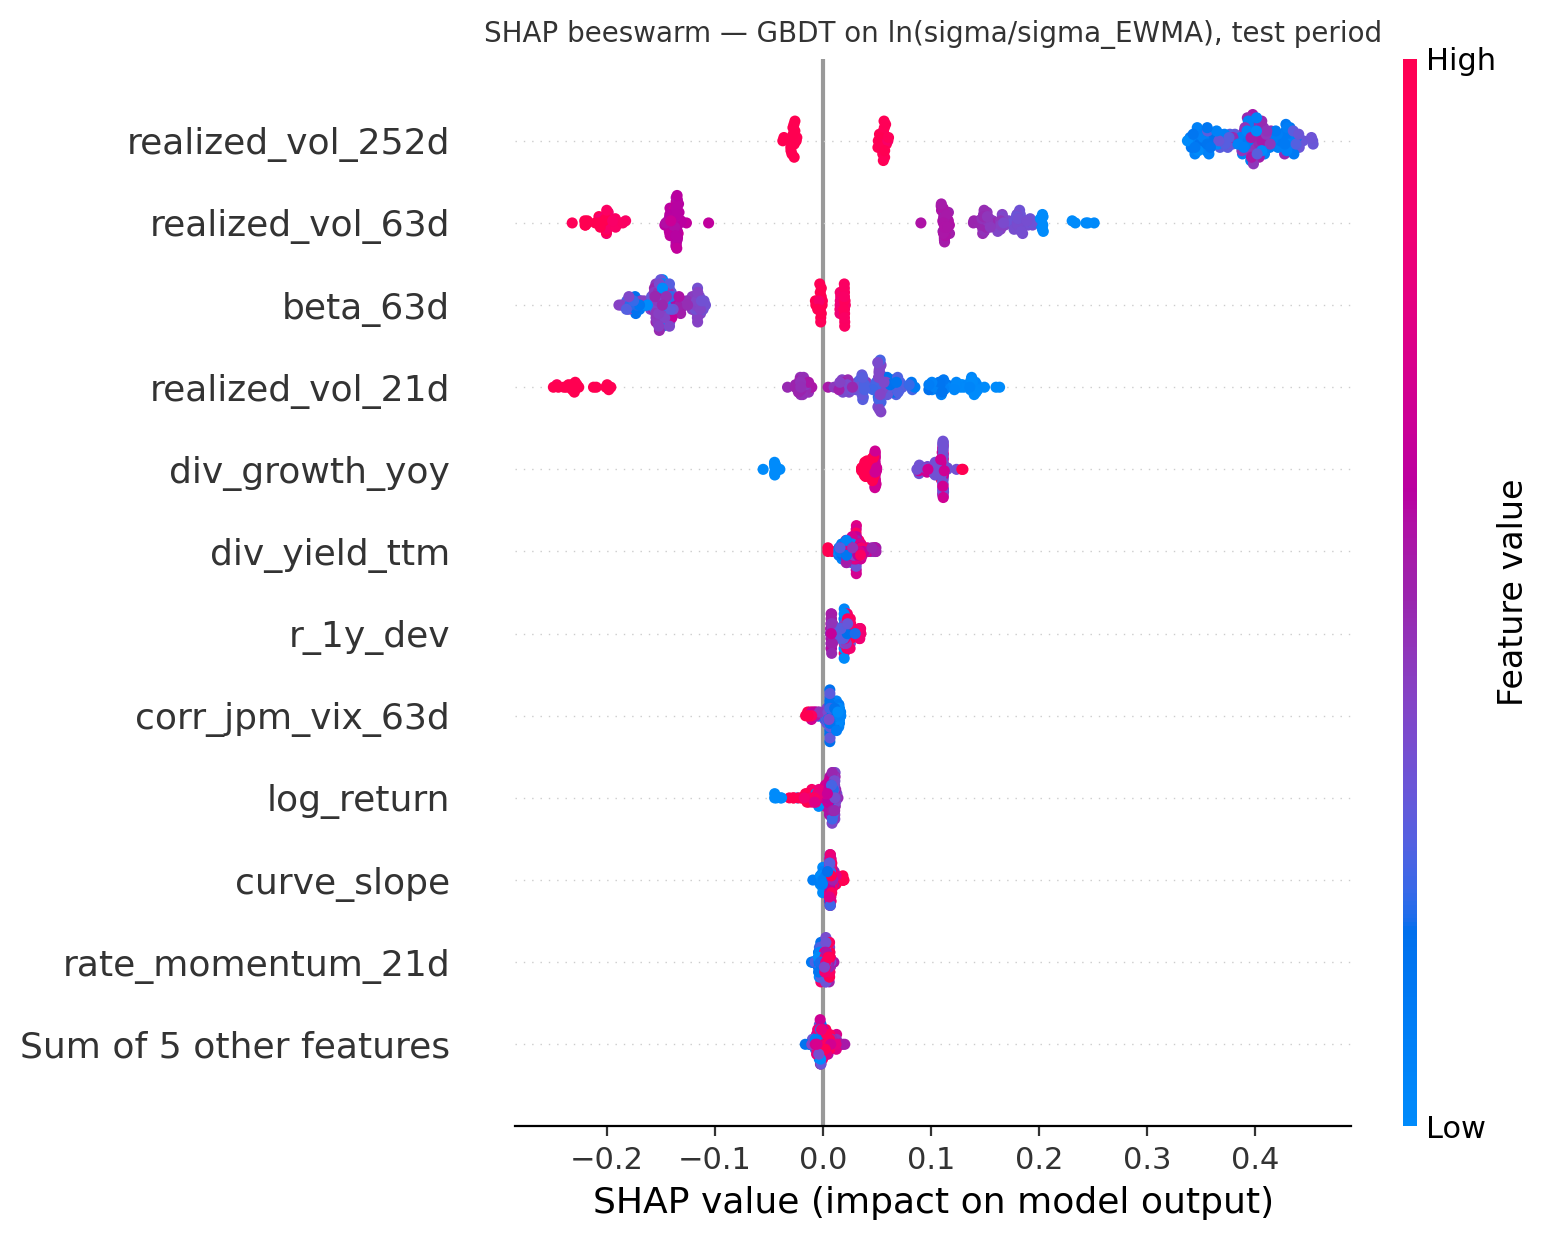
\includegraphics[width=0.66\textwidth]{../week6/figures/shap_beeswarm.png}
\caption{SHAP（部署版 GBDT，锚定目标）：长期已实现波动率主导——当前波动率低于长期水平时模型倾向正修正，干净的均值回复逻辑}
\end{figure}

\section{敏感性分析与定价工具（第 7--8 周）}
以最新市场快照（2026-08-20：$S=\$351.55$、$\sigma_{EWMA}=19.1\%$、$r=3.99\%$）做极端情景：波动率 $+50\%$ $\to$ 价格 $+48.9\%$，而加息 200bp 仅 $+1.5\%$（双腿 vega 叠加、rho 对消——波动率是 chooser 的绝对主导风险因子）；股价 $\pm15\%$ 均抬价（双向凸性）；SHAP 影响经定价函数美元化后，锚定口径下长记忆波动率主导（\texttt{realized\_vol\_252d} 一次典型贡献 $\approx+\$16.9$）。

\textbf{Streamlit 工具}（\texttt{streamlit run app/streamlit\_app.py}）：双定价（主定价 = EWMA 锚定 BSM；ML 参考价附“样本外未证优”警示）、分状态误差区间（第 4 周基准 MAE）、价格趋势、情景与压力面、历史性能指标存档、一键实时数据更新（GitHub Actions 周更为底）。全部定价逻辑位于独立服务层，六项审计通过（与闭式解逐位一致、无套利排序、情景重算、压力面单调、确定性、UI 零公式）。

\begin{figure}[H]
\centering
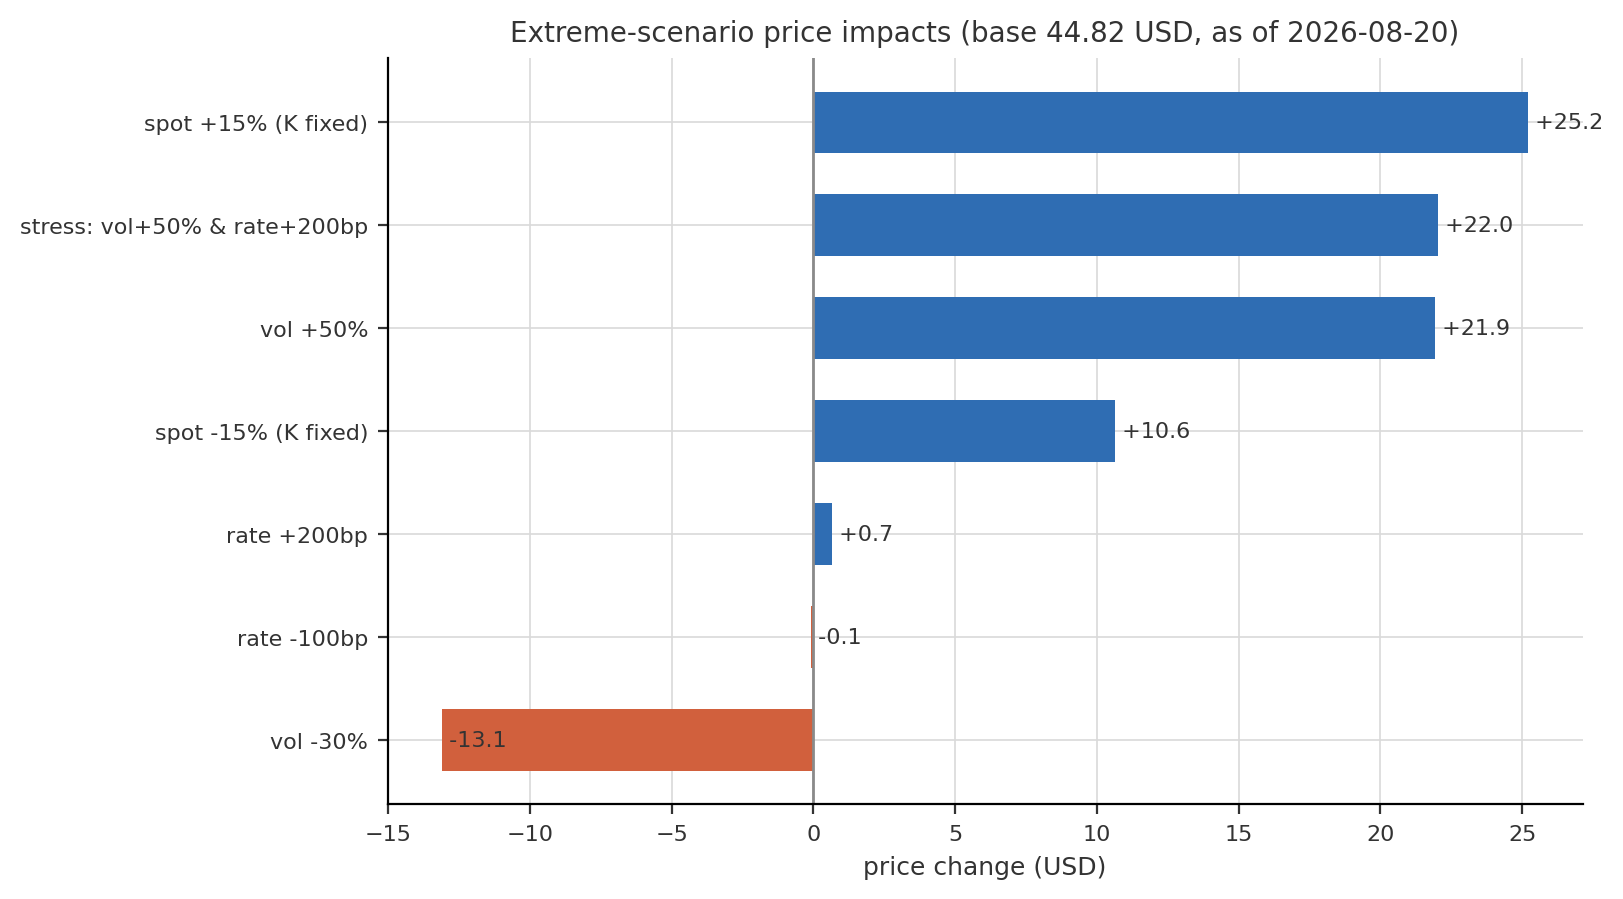
\includegraphics[width=0.74\textwidth]{../week7/figures/scenario_tornado.png}
\caption{极端情景价格冲击（2026-08-20 市场快照，基准 \$44.82）}
\end{figure}

\begin{figure}[H]
\centering
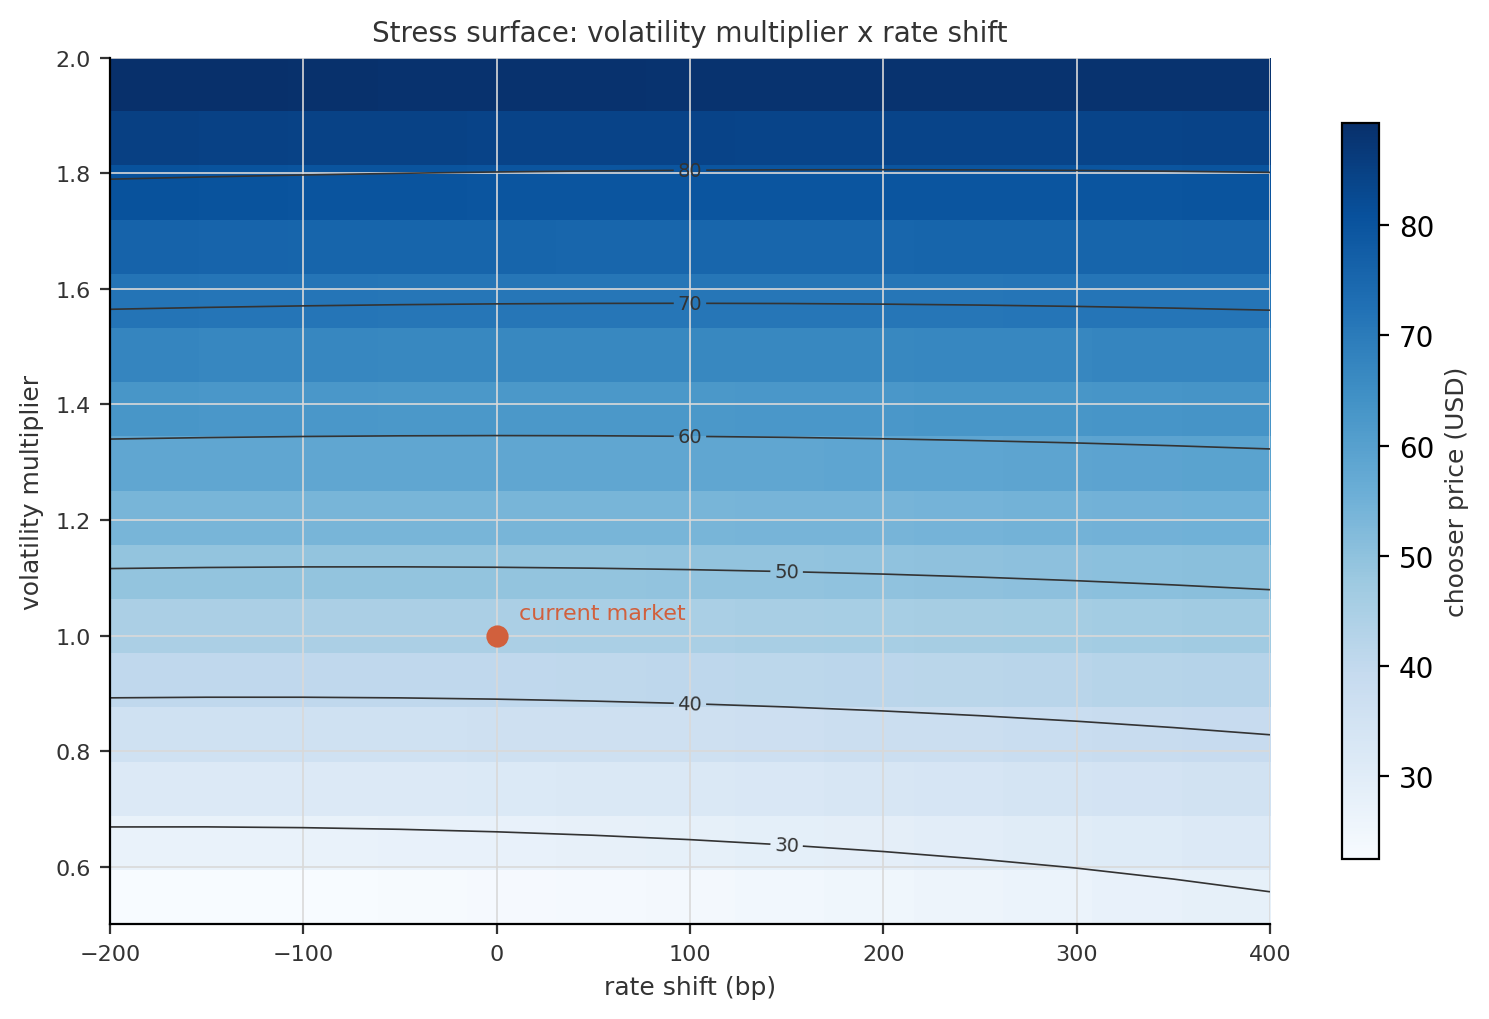
\includegraphics[width=0.68\textwidth]{../week7/figures/stress_heatmap.png}
\caption{压力曲面：波动率乘数 $\times$ 利率平移（等高线为价格）}
\end{figure}

\section{在线架构与运维（第 9 周，第 12 周修复）}
导师对 enhancement 阶段给出三个方向：数据扩展到更大的股票池、接入 SQL 与 Redis 让管道和工具在线运行、测量全流程的时间与空间占用并优化。在线化的验收标准只有一条：\textbf{同一份输入上，新旧两套算术给出相同结果}。

\textbf{架构}：PostgreSQL 存 11 张表（价格、指数、利率、特征、最新状态、成分区间、报价、情景、模型登记、运行日志、证券）；Redis 缓存报价与情景（1 小时有效、按标的失效，不可达时自动降级为直接计算）；调度器在每个交易日收盘后运行日更流水线（增量采集 $\to$ 特征 $\to$ 报价 $\to$ 写库 $\to$ 失效缓存 $\to$ 记录运行日志）；全部服务用 Docker Compose 编排为五个容器（数据库、缓存、一次性迁移、工具、调度器）。第 9 周基线（Apple M4 Pro）：单票报价 \rnWnineQuoteMs{} ms、Redis 命中 \rnWnineRedisMs{} ms、工具首屏 \rnWnineRenderMs{} ms、单票联网日更 \rnWnineDailyS{} s。

\textbf{数据版本}：Yahoo 每次分红后会重算整段复权价，FRED 也会修订近期值，因此“本地快照”与“在线库”是两个数据版本。审计一律在同一版本上比对两套算术；历史报价行视为当日留痕，只断言最新一行可由当前数据复现。

\textbf{第 12 周修复的三个运维缺陷}：
\begin{itemize}
  \item \textbf{调度器漏跑}：宿主机睡眠时 Docker 虚拟机被挂起，调度器计时所用的单调时钟随之停走，一个“51 小时后执行”的等待被不断推迟，导致 9 月 25 日之后没有一次运行，9 月 26 日之后连警告日志都没有。改为每 10 分钟一次心跳，按墙钟判断最近一个应运行时刻之后是否已有成功的日更，没有就立即补跑；心跳文件同时作为调度容器的健康检查（此前它沿用了工具容器的检查，一直显示不健康）。
  \item \textbf{写库会清空未提供的列}：冲突更新原本覆盖全部非主键列，未在本次写入中提供的列会被置空；在给特征表加 GARCH 状态列时发现，改为只更新本次写入实际携带的列。
  \item \textbf{批量特征重建没有逐票容错}：一只标的出错会使整个特征阶段失败（第 12 周实测遇到一次）；改为逐票隔离，出错标的记入运行日志、其余照常写入并定价。
\end{itemize}

\section{全市场扩展与面板研究（第 10 周，第 12 周复核）}
\textbf{点时成分}：由 Wikipedia 当前成分表与历史变更表逆向回放得到 S\&P 500 的成分区间（\rnMemIntervals{} 段、\rnMemTickers{} 只标的）；研究面板逐日只取当日成员，避免用“今天的成分股”回看历史。面板共 \rnPanelTenRows{} 行、\rnPanelTenTickers{} 只。

\textbf{批量化工程}：多源采集（Yahoo 批量 $\to$ Yahoo 单票 $\to$ Alpha Vantage）、增量特征重建（读尾部 760 行、写回 40 行，EWMA 从存量状态续算，与全量重建一致到浮点舍入量级）、向量化全池定价。相对第 9 周逐票路径的倍数：特征重建 \rnEone$\times$、单票状态读取 \rnEtwo$\times$、全池报价 \rnEthree$\times$、全池情景 \rnEfour$\times$；590 只标的日更 \rnTenDailyS{} s，相当于第 9 周单票串行外推的 \rnEfive{} 倍提速。

\textbf{面板上的两项研究}：GARCH 1 日锚在面板上的分标的胜率 \rnGoneDWin\%、池化综合分 \rnGoneDPooled，成为第 11 周的候选锚；锚定 ML 第一轮在验证集全面失败（Ridge 综合分 \rnRoundOneRidge、GBDT \rnRoundOneGbdt），主因是训练窗与验证窗之间面板整体的标签水平漂移——这直接决定了第二轮只学横截面部分（第 \ref{sec:ml2} 节）。

\textbf{数据缺口（第 12 周复核，更正第 10 周的归因）}：研究窗口内曾为成员的 \rnInStudy{} 只标的中，\rnNoPrices{} 只因退市早于采集而没有价格，另有 \rnTruncated{} 只近期退市成员只采到零星的近期数据（数据源不再提供退市股的历史）。研究面板因此带有生存偏差，所有面板结论都应理解为“在样本期内存续的成员”上的结论。另有 \rnPostExit{} 个代码在退出指数后才有价格（代码被其他公司复用，或只采到退出后的片段），已在工具中停用；它们从未进入研究面板（历史不足，或日期不在成员区间内）。第 10 周曾把这类“历史不足”归因于新上市或改名，复核后更正为退市与代码复用。

\section{全流程性能剖析与优化（第 11 周，第 12 周终测）}
第 11 周按导师要求把性能测试提上日程：从仪表板到数据源五层逐层剖析（cProfile、tracemalloc、\texttt{EXPLAIN ANALYZE}、无头渲染），优化前后同一脚本、同一硬件。剖析得出的四个结论直接决定了优化清单：报价慢在 I/O 不在计算；日更有一半时间在等互不依赖的网络请求排队；特征阶段的成本看似在往返次数；首屏里可省的只有表计数。

\begin{center}\small
\begin{tabular}{p{5.2cm}rrr}
\toprule
度量 & 优化前 & 第 11 周优化后 & 第 12 周终测 \\
\midrule
最新状态读取，数据库执行（ms；行数） & \rnLatestBeforeMs（\rnLatestBeforeRows） & -- & \rnLatestFinalMs（\rnLatestFinalRows） \\
全池报价（ms；标的数） & \rnQuBeforeMs（\rnQuBeforeN） & \rnQuAfterMs（\rnQuAfterN） & \rnFinalQuMs（\rnFinalQuN） \\
市场数据阶段（s） & \rnMarketBeforeS & \rnMarketAfterS & -- \\
特征阶段，590 只（s） & \rnFeatBeforeS & \rnFeatAfterS & -- \\
日更，590 只（s） & \rnTenDailyS & \rnDailyAfterS & -- \\
日更，\rnScaleN{} 只稳态（s） & -- & \rnScaleSteadyS & 见正文 \\
工具首屏（ms） & \rnRenderBeforeMs & \rnRenderAfterMs & \rnFinalRenderMs \\
单票报价，未命中缓存（ms） & \rnWnineQuoteMs（第 9 周） & -- & \rnFinalScalarMs \\
数据库（MB） & -- & \rnDbElevenMb & \rnDbFinalMb \\
进程常驻（MB） & -- & \rnRssElevenMb & \rnRssFinalMb \\
\bottomrule
\end{tabular}
\end{center}

\textbf{第 11 周的四项优化}：（O1）每次特征重建时顺手维护一张“最新状态表”，全池报价从扫描整段历史变成按标的数读取；（O2）四个指数与利率并发请求；（O3）特征阶段批量读写，往返次数从每票三次降到每百只三次——\textbf{但阶段时间几乎不变}（\rnFeatBeforeS{} $\to$ \rnFeatAfterS{} s），瓶颈在数据库端的语句执行与滚动算术，这项优化被测量否定，代码保留、结论如实记录；（O4）仪表板用规划器统计代替逐表计数。规模压测把 S\&P 400 与 600 当前成分股加入（只压测、不入研究面板）：\rnScaleN{} 只的首次回填 \rnScaleBackfillS{} s，稳态日更 \rnScaleSteadyS{} s，每票成本随规模下降。

\textbf{第 12 周终测与换锚的代价}：全池报价与单票报价变慢，是因为新的 ML 参考价需要当日整个截面（横截面计算本身 \rnFinalXsMs{} ms），Redis 命中路径不受影响。GARCH 锚给日更增加一个步骤，按内存模拟（\rnGarchTickers{} 只、不写库）：普通交易日 \rnGarchOrdS{} s；重估日 \rnGarchRefitS{} s。重估按“第几个收益”排程，而大多数标的的历史从同一天开始，于是 \rnGarchRefits{} 只在同一天重估，形成每 21 个交易日一次的尖峰；为不改变经过检验的 GARCH 定义，没有错开排程。普通日不再读取完整收益历史，只从存量状态续算（与全量计算逐位一致，审计断言）。换锚后第一次日更补了 6 个交易日（\rnCatchupS{} s，其中特征阶段 \rnCatchupFeatS{} s），不是稳态口径；稳态的实测以调度器之后的正常运行为准。数据库在一次性回填后曾因旧版本行膨胀，表中数字为整理（VACUUM FULL）之后的大小。

\section{锚定机器学习第二轮与统计显著性（第 11--12 周）}\label{sec:ml2}
\subsection{第二轮设计与第 11 周的测试}
第一轮的失败来自面板整体的水平漂移，第二轮因此只学修正的\textbf{横截面}部分：目标按日期去均值，特征在每个日期内标准化，锚改用 GARCH 1 日预测；定价时 $\sigma_{ml}=\sigma_{anchor}\,e^{\hat y}$。验证集选型（综合分 \rnElevenVal），测试集自 \rnElevenTestStart{} 起开封一次：GARCH 锚加横截面 GBDT 综合分 \rnElevenTestMl，GARCH 锚单独 \rnElevenTestG，EWMA 为 1.000（MAE \rnElevenMaeMl{} / \rnElevenMaeG{} / \rnElevenMaeE{} 美元）。大部分收益来自换锚，ML 在其上再进一步。

第 11 周复检补充了三项诊断（开封之后做，不用于选择）：（1）行业哑变量取自当前成分表，记为“未知行业”的 \rnUnknownN{} 只中 \rnUnknownRemoved{} 只后来被移出指数，带有前视；去掉行业哑变量后测试集综合分 \rnNoDummyTest，结果没有被抬高，部署版因此不用行业哑变量。（2）提名 GARCH 锚的第 10 周面板评估已包含测试期，换锚的测试前证据是训练期 \rnGTrain{} 与验证期 \rnGVal。（3）把修正拆成两部分单独使用：只保留同日内重排 \rnCsOnly，只保留水平平移 \rnLevelOnly{}（比不修正还差）——收益全部来自横截面。

\subsection{第 12 周：显著性边界（回应导师）}
导师要求给出 ML 增量的统计显著性边界。在跑任何新数之前，检验判据写入 \url{docs/week12/preregistration.json} 并记录其 SHA-256：
\begin{itemize}
  \item \textbf{样本}：第 11 周模型（去掉行业哑变量）在全部 walk-forward 区块上的样本外预测，自第一个“净化后训练集不少于 252 个日期”的区块起，至 2024-12-31。
  \item \textbf{统计量与推断}：两模型的美元 MAE 之差；按股票整簇重抽样的 bootstrap（2000 次）给 95\% 区间——推断\textbf{以实际经历的时间路径为条件}，回答的是“在这段时期内，增量是否普遍存在于各只股票”。
  \item \textbf{先查程序是否合格}：每个假设都用它自己的损失差拟合出“行业共同冲击 + 个股噪声”的相依结构，在均值为零的模拟面板上检验 5\% 名义水平的实际拒绝率，只采用落在 2.5\%--7.5\% 之间的程序；按股票的程序不合格时改用“先抽行业、再抽股票”的程序并同样检验，两者都不合格则只作描述。
  \item \textbf{族与矫正}：换锚（H1）、ML 增量（H2）、隐含波动率对 GARCH 1 日锚（H3）、隐含波动率对免费平稳锚（H4）四项一起做 Holm 矫正；时间维度按日历年描述，一年期标签下独立年份太少，\textbf{不给时间维度的 p 值}。
\end{itemize}
size 检验本身也是自写的程序，先在已知答案的数据上验证：纯独立噪声下按股票的程序拒绝率 \rnSelfIidTicker\%；加入很强的行业冲击后它升到 \rnSelfShockTicker\%（被正确识别为失准），行业簇程序为 \rnSelfShockSector\%——行业只有 12 簇，在极端相依下行业簇程序也会略偏宽松，因此逐个假设检验、只取合格者，而不是默认某个程序可用。

\begin{center}\small
\begin{tabular}{p{5.3cm}rrrrl}
\toprule
假设（$\Delta$MAE，美元） & 估计 & 95\% 区间 & 按股票 size & 按行业 size & 结论 \\
\midrule
H1 换锚（EWMA $\to$ GARCH 1 日） & \rnHOneDelta & \rnHOneLo--\rnHOneHi & \rnHOneSizeTicker\% & \rnHOneSizeSector\% & 仅描述 \\
H2 ML 增量（主假设） & \rnHTwoDelta & \rnHTwoLo--\rnHTwoHi & \rnHTwoSizeTicker\% & \rnHTwoSizeSector\% & 显著 \\
H3 隐含波动率 vs GARCH 1 日 & \rnHThreeDelta & \rnHThreeLo--\rnHThreeHi & \rnHThreeSizeTicker\% & \rnHThreeSizeSector\% & 显著 \\
H4 隐含波动率 vs GARCH 1 年 & \rnHFourDelta & \rnHFourLo--\rnHFourHi & \rnHFourSizeTicker\% & \rnHFourSizeSector\% & 仅描述 \\
\bottomrule
\end{tabular}
\end{center}
注：区间来自行业簇程序（四项假设上按股票的程序全部严重失准）；显著者的 Holm 校正 p 值为 \rnHTwoPholm（bootstrap 的最小可分辨值）。H1、H2 的样本外窗口为 \rnOosStart{} 至 \rnOosEnd（\rnOosDates{} 个交易日、\rnOosRows{} 行、\rnOosTickers{} 只；MAE：EWMA \rnOosMaeE、GARCH 1 日 \rnOosMaeG、加 ML \rnOosMaeMl）。

\textbf{读数}：（1）ML 增量为每份 \rnHTwoDelta{} 美元 MAE，95\% 区间 \rnHTwoLo--\rnHTwoHi，在这段时期内显著且普遍存在于各只股票；但它主要来自 2024 年（\rnHTwoYFour），2023 年只有 \rnHTwoYThree，而独立的一年期窗口只有两个，时间维度上不能推断它会在别的年份重现。（2）带行业哑变量的第 11 周原模型增量为 \rnHTwoBDelta，低于部署版，与前视诊断一致。（3）换锚的估计增量（\rnHOneDelta{} 美元）远大于 ML 增量，且在每个合格年份都为正，但它的推断程序 size 不合格，按事先规则只作描述——这不推翻第 11 周换锚的决定（训练、验证、测试三个窗口均占优），只是不能给它贴“统计显著”的标签。（4）按事先规则，ML 增量判定成立，ML 参考价从 JPM 扩展到面板成员（第 \ref{sec:tool} 节）。

\begin{figure}[H]
\centering
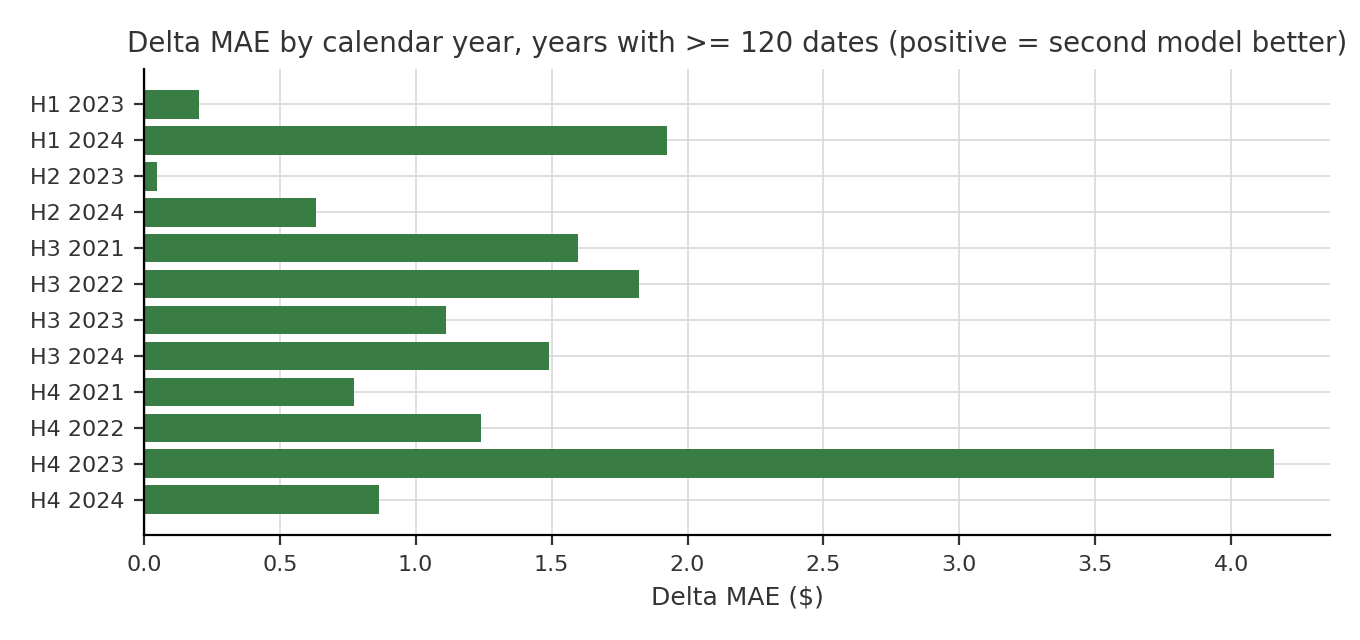
\includegraphics[width=0.78\textwidth]{figures/increment_by_year.png}
\caption{各假设的逐年 $\Delta$MAE（只画样本外交易日不少于 120 天的年份；正值表示后者更好），描述性}
\end{figure}

\section{隐含波动率的定位（第 11--12 周）}\label{sec:iv}
导师的第二个问题是隐含波动率是否值得作为候选锚。数据为 OptionMetrics 365 天、$|\Delta|=50$ 的隐含波动率（看涨看跌均值），按学校 WRDS 许可只在本机做研究、不进入工具与交付物，图表只画派生结果。证券代码会被复用或更名，因此只按“与本地价格的日收益相关系数不低于 0.98”的规则匹配证券。

\textbf{第 11 周的 JPM 读数需要修正}：当时引用的“隐含波动率与 EWMA 修正量相关 \rnIvJpmCorr”是机械相关——两边都含 $-\ln\sigma_{EWMA}$，把隐含波动率换成一个常数，相关系数反而是 \rnIvJpmCorrConst。它在 JPM 上的综合分 \rnIvJpm{} 本身成立。

\textbf{面板证据}（\rnIvPanelTickers{} 只、\rnIvPanelRows{} 行，五个锚都可用的共同样本）：MAE 隐含波动率 \rnIvMaeIv、GARCH 1 日 \rnIvMaeGd、GARCH 1 年 \rnIvMaeGy、252 日已实现 \rnIvMaeRv、EWMA \rnIvMaeEw{} 美元；隐含波动率在 \rnIvWinGd\% 的股票上胜过 GARCH 1 日锚、在 \rnIvWinGy\% 上胜过 GARCH 1 年锚。对 GARCH 1 日锚的优势显著（H3）；对免费平稳锚 GARCH 1 年锚的优势估计为 \rnHFourDelta{} 美元、逐年为正，但推断程序 size 不合格，只作描述（H4）。

\textbf{优势从哪里来}（描述性诊断，含前视）：把隐含波动率与 GARCH 1 年锚都换成“各自在每只股票上的样本均值”这一常数后，两者的 MAE 差距几乎不变（\rnIvGapConst{} 对 \rnIvGapActual{} 美元）；隐含波动率的每股均值与事后真值的横截面相关为 \rnIvXsIv（GARCH 1 年锚 \rnIvXsGy），而它在时间上与事后真值相关的中位数只有 \rnIvTsIv。因此在面板上，隐含波动率的优势来自\textbf{对每只股票波动率水平的定位}，而不是择时——第 11 周在 JPM 一只股票上“赢在平稳”的读法，在面板上应修正为“赢在横截面水平”。

\textbf{定位（按预注册判据）}：\textbf{研究基准，不列为候选锚}。理由有二：对免费平稳锚的优势未能通过合格的推断程序；可部署性无法核实——OptionMetrics 数据截至 2025-08-29，公开的 Yahoo 期权链只有当日快照，两者没有同一天可以对照。由此给出的方向是：用隐含波动率给出的水平去设定 GARCH 的长期方差（方差目标化），让随机过程的锚继承期权市场对水平的判断，同时保留 GARCH 的可部署性。

\begin{figure}[H]
\centering
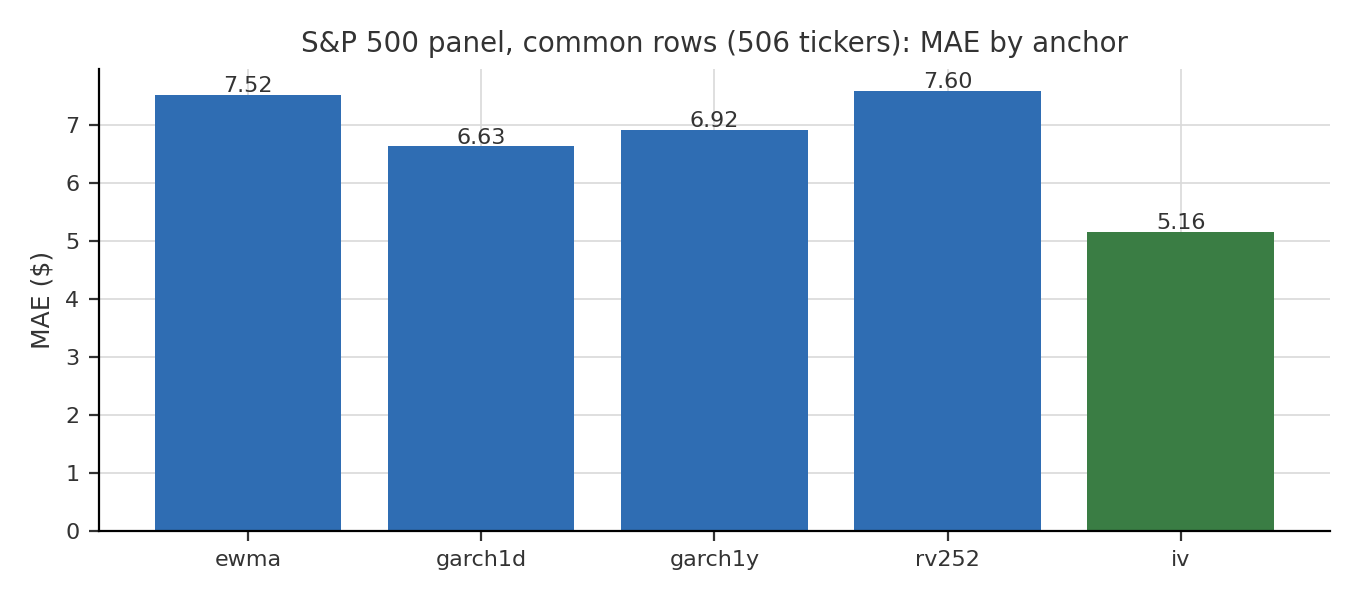
\includegraphics[width=0.72\textwidth]{figures/iv_panel_mae.png}
\caption{S\&P 500 面板共同样本上各锚的 MAE（不含隐含波动率序列本身）}
\end{figure}

\section{工具的最终形态（第 12 周）}\label{sec:tool}
\begin{itemize}
  \item \textbf{主定价锚换为 GARCH(1,1) 1 日预测}：每只股票逐日存储 GARCH 的参数与条件方差，日更时从存量状态续算、到排定日才重估；与研究所用的定义逐位一致（同一平台内；GARCH 参数靠数值优化求得，macOS 与 Linux 容器的优化器会停在似然面上略有不同的点：用于定价的 $\sigma$ 审计以相对 $10^{-4}$ 容差断言一致，参数本身以 $10^{-2}$）。历史不足 750 个交易日的新股没有 GARCH 状态，逐行退回 EWMA，每笔报价都标明所用的锚：截至 \rnToolAsOf，\rnToolQuoted{} 笔报价中 \rnToolGarch{} 笔用 GARCH、\rnToolEwma{} 笔用 EWMA。
  \item \textbf{误差区间}：沿用第 4 周的定义（JPM 上按市场状态的定价 MAE）。GARCH 锚为平静 \rnBandGCalm{} / 恐慌 \rnBandGFear{} 美元，但 GARCH 需要 750 个观测，校准窗口只有 \rnBandGDays{} 天（2020-12 至 2024-12），不含 2020 年崩盘；同一窗口上 EWMA 为 \rnBandESameCalm{} / \rnBandESameFear，原 EWMA 带宽为 \rnBandEFullCalm{} / \rnBandEFullFear。区间变窄主要来自窗口而非换锚，危机中可能偏窄，工具界面已注明。
  \item \textbf{ML 参考价}：横截面 GBDT（GARCH 锚、无行业哑变量），在第 11 周研究面板上固化；适用范围为报价当日的点时 S\&P 500 成员且有 GARCH 锚（\rnToolMl{} 只），范围外不做外推；替代原先只覆盖 JPM、以 EWMA 为基的第 6 周 Ridge。
  \item \textbf{兼容}：\texttt{PRIMARY\_ANCHOR=ewma} 可切回 EWMA 主定价；第 7、9--11 周的审计全部保留并通过（其中与主锚或 ML 范围相关的断言已随换锚同步修改），第 12 周新增 12 项审计。
\end{itemize}

\section{结论与展望：机器学习 $\times$ 随机过程的 1+1 融合}
本项目的全部证据指向同一个结构性结论：\textbf{随机过程与机器学习不是竞争关系，而是分工关系}——前者负责无套利框架、可对冲体系与可归因的误差结构，后者负责框架内解析方法覆盖不到的残差。据此提出五条融合路线（按可行性排序）：
\begin{enumerate}
  \item \textbf{锚定残差学习（本项目已实践）}：ML 预测 $\ln(\sigma/\sigma_{anchor})$ 而非水平，输出经 BSM 映射自动满足无套利；表现有基线下界。当前数据规模下修正幅度不可稳健标定，但框架正确——数据条件（多周期历史或个股隐含波动率）满足时即可释放；
  \item \textbf{收缩融合}：$\sigma = \sigma_{anchor}\cdot e^{\lambda \hat y}$，收缩系数 $\lambda\in[0,1]$ 由滚动验证标定——在“完全信任锚”与“完全信任 ML”之间连续插值，最坏情形受控；
  \item \textbf{状态门控校准}：ML 不直接定价，而判别当前波动率状态（平静/恐慌/转换），据此切换随机过程侧的校准窗口——直接针对第 4 周“无单一窗口全状态占优”的发现，ML 只做它擅长的分类；
  \item \textbf{隐含波动率曲面残差}：以随机过程模型（SVI/局部波动率）拟合个股期权隐含波动率曲面，ML 学习曲面残差的动态——信息含量与样本量均优于时序外推，是解除本项目数据约束的首选（需个股期权数据）；
  \item \textbf{ML 作定价加速器（surrogate）}：训练数据由随机过程模型自身生成（要多少有多少，无信噪比问题），ML 学习“参数 $\to$ 价格”映射以加速复杂模型（随机波动率、美式 chooser）的实时定价与校准——与市场有效性无冲突，工程价值确定。
\end{enumerate}
其中 4、5 与美式 chooser（Longstaff--Schwartz）共同构成 enhancement 阶段的候选方向。

\textbf{第 9--12 周之后的回看}：路线 1（锚定残差学习）在换用更强的锚、并且只学横截面之后，第一次在样本外给出了有边界的正增量（第 \ref{sec:ml2} 节）；同一组样本上，换锚带来的改进约为 ML 增量的三倍（\rnHOneDelta{} 对 \rnHTwoDelta{} 美元）——随机过程负责水平，机器学习负责同一天内股票之间的相对差异，这是“1+1 分工”的实证形态。路线 4（隐含波动率）在面板上给出了最强的单一证据，但它的价值在于水平定位，当前的许可与数据源使它只能作为研究基准（第 \ref{sec:iv} 节）。留给后续的方向：用隐含波动率做 GARCH 的方差目标化；更长的样本外历史（时间维度上的显著性需要更多独立年份）；美式 chooser 与 ML 加速器（路线 5）。

\section*{附录：可复现性}
全流程固定种子、重跑逐位一致；每周交付经固定自检套餐（确定性重跑、审计断言、依赖扫描、打包泄露检查、报告数字回查）；逐周审计脚本位于 \url{analysis/weekN/}；一键复现入口 \texttt{python -m src.analysis\_w3} 至 \texttt{w7}；数据管道 \texttt{python -m src.collect\_all} + \texttt{src.preprocess}；部署模型 \url{models/final_*.joblib}。代码仓库结构与运行说明见 README。

\textbf{第 9--12 周补充}：在线栈一键启动 \texttt{docker compose up -d}；理论线入口为 \url{src/analysis_w9.py} 至 \url{src/analysis_w12.py}（以 \texttt{python -m} 模块方式运行），审计脚本位于 \url{analysis/week9} 至 \url{analysis/week12}（第 12 周审计会连带回归第 7、9--11 周）。第 12 周的检验判据在跑数前写入 \url{docs/week12/preregistration.json}，其 SHA-256 存于同目录并由审计核对；本报告第 7--12 节的全部数字由 \url{analysis/week12/04_report_numbers.py} 从各周输出生成（\url{numbers.tex}，来源逐项列于 \url{numbers_sources.csv}），数据库中的计时与覆盖统计冻结在 \url{db_snapshot.json}。逐位复现成立的范围是“同一份数据、同一平台”：数据源会修订历史，GARCH 优化器的末几位在 macOS 与 Linux 上不同。OptionMetrics 提取文件仅在作者本机，不随代码分发，相关脚本在无该文件时自动跳过。

\section*{附录：GenAI 使用情况说明}
\textbf{使用的工具}：本项目使用 Anthropic Claude Code 作为编程与写作助手在本地终端中运行，无其他生成式 AI 工具。

\textbf{使用范围}：AI 参与了以下工作的初稿或实现：
\begin{enumerate}
  \item 代码实现：数据采集与清洗脚本、BSM 与 chooser 定价模块、蒙特卡洛验证、评估指标模块、机器学习训练与 walk-forward 协议、情景引擎、Streamlit 工具及各周审计脚本；
  \item 文档排版与初稿：周报、学习报告、各周技术文档、最终报告、演示幻灯的 LaTeX 与 pptx 生成，以及图表绘制脚本；
  \item 工程辅助：调试、依赖检查、交付物打包、格式修正（如中文标点统一、拼写标记清理）、录屏拼接；
  \item 第 9--12 周：在线栈（PostgreSQL、Redis、Docker）、全市场扩展与性能剖析的实现，显著性检验与预注册文件、结项报告续写的初稿。
\end{enumerate}

\textbf{由本人完成的部分}：
\begin{enumerate}
  \item 参考资料的选择：除了导师推荐的书目外，还新添了自己学过看过的一些随机过程、时间序列、数值方法等的书籍作为参考；
  \item 问题定义与阶段规划：在给定的框架下确定每周的具体范围与推进节奏；
  \item 关键方法的提出或决策：验证方式改为蒙特卡洛和情绪数据改用 VIX（这两者由本人提出并交给导师拍板）、锚定目标的采纳、测试集只开封一次的协议、第六周负结果的如实报告（而非继续调参）等；
  \item 与导师的全部沟通，以及根据导师反馈对方向和材料形态的调整；
  \item 结果审查：对 AI 产出的代码逻辑、报告数字与图表口径逐项核对，发现并要求修正过多处不一致（如第八周幻灯中的图表与讲述口径的不一致、报告图表数量不足等）；
  \item 演示视频的讲解与录制，以及学习报告初版（项目启动前撰写的那部分）中的问题设定。
\end{enumerate}

\textbf{质量控制方式}：为了防止 AI 生成内容引入错误，本项目建立了固定的自检流程：
\begin{itemize}
  \item 每周所有分析脚本都使用固定的随机种子重跑并逐位比对；
  \item 每周编写独立的审计脚本、检查重要的性质（如闭式解与蒙特卡洛一致、锚定模型输出零时恒等于基线、工具与研究代码统一口径）；
  \item 用静态扫描核对依赖列表；
  \item 将报告中的每个数字都回查到生成它的脚本输出（两套独立实现的闭式解在 $7\times10^{-15}$ 精度上一致就是这一流程的一个例子）；
  \item 第 12 周起：检验判据先登记后跑数，自写的统计程序先在已知答案的数据上验证，报告数字由脚本生成为宏；交付前的复查按“冻结后只修实质错误、最后只查增量”收敛。
\end{itemize}

\section*{参考文献}
\begin{enumerate}
  \item Huang, Z., Wang, X., Wan, W. (2021). \textit{Exploration of JPMorgan Chooser Option Pricing}. BCP Business \& Management, Vol.~15, 93--102.（复现对象）
  \item Rubinstein, M. (1991). \textit{Options for the Undecided / Exotic Options}.（simple chooser 闭式解）
  \item Hull, J., White, A. (1987). \textit{The Pricing of Options on Assets with Stochastic Volatilities}. Journal of Finance.（常数波动率局限）
  \item Gu, S., Kelly, B., Xiu, D. (2020). \textit{Empirical Asset Pricing via Machine Learning}. RFS.（金融 ML 方法论）
  \item Bakshi, G., Cao, C., Chen, Z. (1997). \textit{Empirical Performance of Alternative Option Pricing Models}. Journal of Finance.（替代模型基准）
  \item Hull, J. \textit{Options, Futures, and Other Derivatives}，11th ed.（理论底本）
  \item Bollerslev, T. (1986). \textit{Generalized Autoregressive Conditional Heteroskedasticity}. Journal of Econometrics.（GARCH 锚）
  \item J.P. Morgan / Reuters (1996). \textit{RiskMetrics --- Technical Document}, 4th ed.（EWMA，$\lambda=0.94$）
  \item Holm, S. (1979). \textit{A Simple Sequentially Rejective Multiple Test Procedure}. Scandinavian Journal of Statistics.（多重比较矫正）
  \item Cameron, A. C., Gelbach, J. B., Miller, D. L. (2008). \textit{Bootstrap-Based Improvements for Inference with Clustered Errors}. Review of Economics and Statistics.（整簇 bootstrap）
  \item OptionMetrics. \textit{IvyDB US Reference Manual}.（波动率曲面数据，经 WRDS 访问）
\end{enumerate}
\end{document}
